\section{\normalsize \textit{BUCKET SORT}}\label{bucket}
	O \textit{Bucket sort} é uma técnica de classificação que classifica os elementos primeiro os dividindo em vários grupos chamados baldes\footnote{ou \textit{buckets} em inglês, daí o nome.}. Os elementos dentro de cada grupo são classificados usando qualquer um dos algoritmos de classificação adequados ou chamando recursivamente o mesmo algoritmo.

Vários \textit{buckets}\footnote{deste ponto em diante, o termo \textit{bucket} será utilizado ao invés do termo balde.} são criados. Cada \textit{bucket} é preenchido com um intervalo específico de elementos, que então são  classificados usando qualquer outro algoritmo. Por fim, os elementos de cada \textit{bucket} são reunidos para obter a matriz ou o vetor original classificado.

O processo de classificação pode ser entendido como uma abordagem de coleta dispersa. Os elementos são primeiro dispersos em \textit{buckets} e, em seguida, os elementos dos \textit{buckets} são classificados. Finalmente, os elementos são reunidos em ordem.

Esse algoritmo é especialmente útil, e fácil de implementar, em aplicações paralelas, onde cada \textit{bucket} pode ser enviado para um processo, onde o mesmo ordenará o \textit{bucket} e o reenviará, já ordenado, para o processo de origem, o que poderá, dependendo de uma série de fatores, acarretar em um aumento de desempenho com relação à sua implementação sequencial.

	\subsection{\normalsize CLASSIFICAÇÃO DOS \textit{BUCKETS}}\label{classification}
		Os elementos podem ser classificados através de uma função matemática que, dados os valores máximos e mínimos dos elementos, além do número de \textit{buckets} disponível, determina para qual \textit{bucket} tal elemento será enviado.
		
		Essa classificação, apesar de adicionar mais processamento ao algoritmo, garante que, após a ordenação de todos os \textit{buckets}, ao agrega-los, do \textit{bucket} de menor índice (0) até o maior (\textit{n}), o vetor já se encontre ordenado, uma vez que cada \textit{bucket} conterá  um intervalo de elementos que sempre será superior ao \textit{bucket} anterior\footnote{com exceção do \textit{bucket} 0} e inferior ao \textit{bucket} seguinte\footnote{com exceção do último \textit{bucket}}.
		
		As imagens a seguir ilustram melhor isso:
		\begin{figure}[H]
			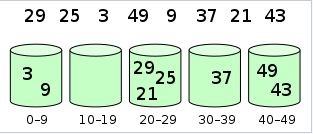
\includegraphics[scale=1]{pictures/01}
		\end{figure}
		
		\begin{figure}[H]
			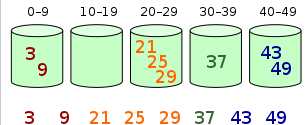
\includegraphics[scale=1]{pictures/02}
		\end{figure}
		
		A função matemática que é usada para calcular em qual \textit{bucket} o elemento deve ser inserido é:
		$$\cfrac{elem - min}{\frac{max - min + 1}{buckets}}$$
		
		Onde:
		\begin{itemize}
			\item elem: é o elemento que se deseja inserir em algum \textit{bucket};
			\item min: menor elemento presente no vetor ou matriz;
			\item max: maior elemento presente no vetor ou matriz e
			\item buckets: número total de \textit{buckets} existentes.
		\end{itemize}
		
	\subsection{\normalsize COMPLEXIDADE}\label{complex}
		\begin{itemize}
			\item \textbf{Pior Complexidade ($\theta(n^{2})$)}:\\
				Quando a distribuição dos elementos não for uniforme, os mesmos provavelmente serão colocados no mesmo \textit{bucket}. Isso pode resultar em alguns \textit{buckets} com mais número de elementos do que outros, o que irá atrasar a execução consideravelmente.
				
				Nesse cenário, a complexidade passa a depender do algoritmo de ordenação usado para ordenar os elementos do \textit{bucket}.
				
				A complexidade se torna ainda pior quando os elementos estão na ordem inversa.
			
			\item \textbf{Melhor Complexidade ($\theta(n + k)$)}:\\
				Ocorre quando os elementos são distribuídos uniformemente nos \textit{buckets}, com um número quase igual de elementos em cada \textit{bucket}.
				
				A complexidade se torna ainda melhor se os elementos dentro dos \textit{buckets} já estiverem classificados.

				Se o algoritmo de ordenação utilizado for de tempo linear, a complexidade geral, na melhor das hipóteses, será linear, isto é, $\theta(n + k)$, onde $\theta(n)$ representa a complexidade para inserir os elementos nos \textit{buckets} e $\theta(k)$ representa a complexidade para ordenar os elementos do \textit{bucket}\footnote{considerando que os algoritmos usados são de complexidade de tempo linear}.
				
			\item \textbf{Caso Médio ($\theta(n)$)}:\\
				Isso ocorre quando os elementos são distribuídos aleatoriamente na matriz. Mesmo que os elementos não sejam distribuídos uniformemente, a classificação do \textit{bucket} é executada em tempo linear.
		\end{itemize}